% ── Section 7: Analysis ───────────────────────────────────────────────────────
\section{Analysis}
\label{sec:analysis}

\subsection{Error Type Analysis}

Table~\ref{tab:error_types} breaks down WER into substitution (S), deletion
(D), and insertion (I) rates, and reports English word survival rate for CS
clips.

\begin{table}[h]
\centering
\caption{Error type breakdown and English word survival rate.
S/D/I = substitution/deletion/insertion as fraction of reference words.
EN-Surv = fraction of English reference words found in hypothesis.}
\label{tab:error_types}
\small
\begin{tabular}{lrrrrr}
\toprule
\textbf{Model} & \textbf{S} & \textbf{D} & \textbf{I} & \textbf{EN-Surv}$\uparrow$ \\
\midrule
Whisper large-v3 (0-shot) & \TODO{0.XX} & \TODO{0.XX} & \TODO{0.XX} & \TODO{0.XX} \\
Tugstugi/whisper-bn       & \TODO{0.XX} & \TODO{0.XX} & \TODO{0.XX} & \TODO{0.XX} \\
MMS-1B                    & \TODO{0.XX} & \TODO{0.XX} & \TODO{0.XX} & \TODO{0.XX} \\
wav2vec2 (zero-shot)      & \TODO{0.XX} & \TODO{0.XX} & \TODO{0.XX} & \TODO{0.XX} \\
\midrule
wav2vec2 FT (no LM)       & \TODO{0.XX} & \TODO{0.XX} & \TODO{0.XX} & \TODO{0.XX} \\
wav2vec2 FT + LM          & \TODO{0.XX} & \TODO{0.XX} & \TODO{0.XX} & \TODO{0.XX} \\
WavLM FT (no LM)          & \TODO{0.XX} & \TODO{0.XX} & \TODO{0.XX} & \TODO{0.XX} \\
WavLM FT + LM             & \TODO{0.XX} & \TODO{0.XX} & \TODO{0.XX} & \TODO{0.XX} \\
\midrule
Whisper FT BN\_ONLY (A)   & \TODO{0.XX} & \TODO{0.XX} & \TODO{0.XX} & \TODO{0.XX} \\
Whisper FT CS\_ONLY (B)   & \TODO{0.XX} & \TODO{0.XX} & \TODO{0.XX} & \TODO{0.XX} \\
\BEST{Whisper FT ALL}     & \BEST{\TODO{0.XX}} & \BEST{\TODO{0.XX}} & \BEST{\TODO{0.XX}} & \BEST{\TODO{0.XX}} \\
\bottomrule
\end{tabular}
\end{table}

\paragraph{English word deletion.}
A key finding is that CTC models without LM fusion exhibit high English word
\emph{deletion} rates (\TODO{XX.X}\%).
This occurs because the acoustic model has learned to ignore acoustically
ambiguous English words (which may sound like Bengali words to a model not
trained on CS) and produces only Bengali output.
LM shallow fusion substantially reduces this deletion rate by encouraging the
model to output English words where the context suggests it.
The proposed Whisper FT ALL model achieves the highest English word survival
rate (\TODO{XX.X}\%), demonstrating that seq2seq models with a shared
multilingual vocabulary handle CS words more faithfully.

\paragraph{Substitution patterns.}
The most frequent substitution errors involve:
(1)~dialect-specific phonemes being substituted with standard Bengali
equivalents (e.g., Chittagong /\textipa{Ef}/ $\to$ /\textipa{E}/);
(2)~English technical terms being transcribed in Bengali script
(transliteration rather than transcription); and
(3)~short English function words (``is'', ``the'', ``in'') being deleted.

\subsection{Cross-Dialect Generalisation}

Figure~\ref{fig:cross_dialect} shows the leave-one-dialect-out (LODO) WER
for selected dialects, comparing models trained with vs.\ without the
target dialect.

\begin{figure}[h]
\centering
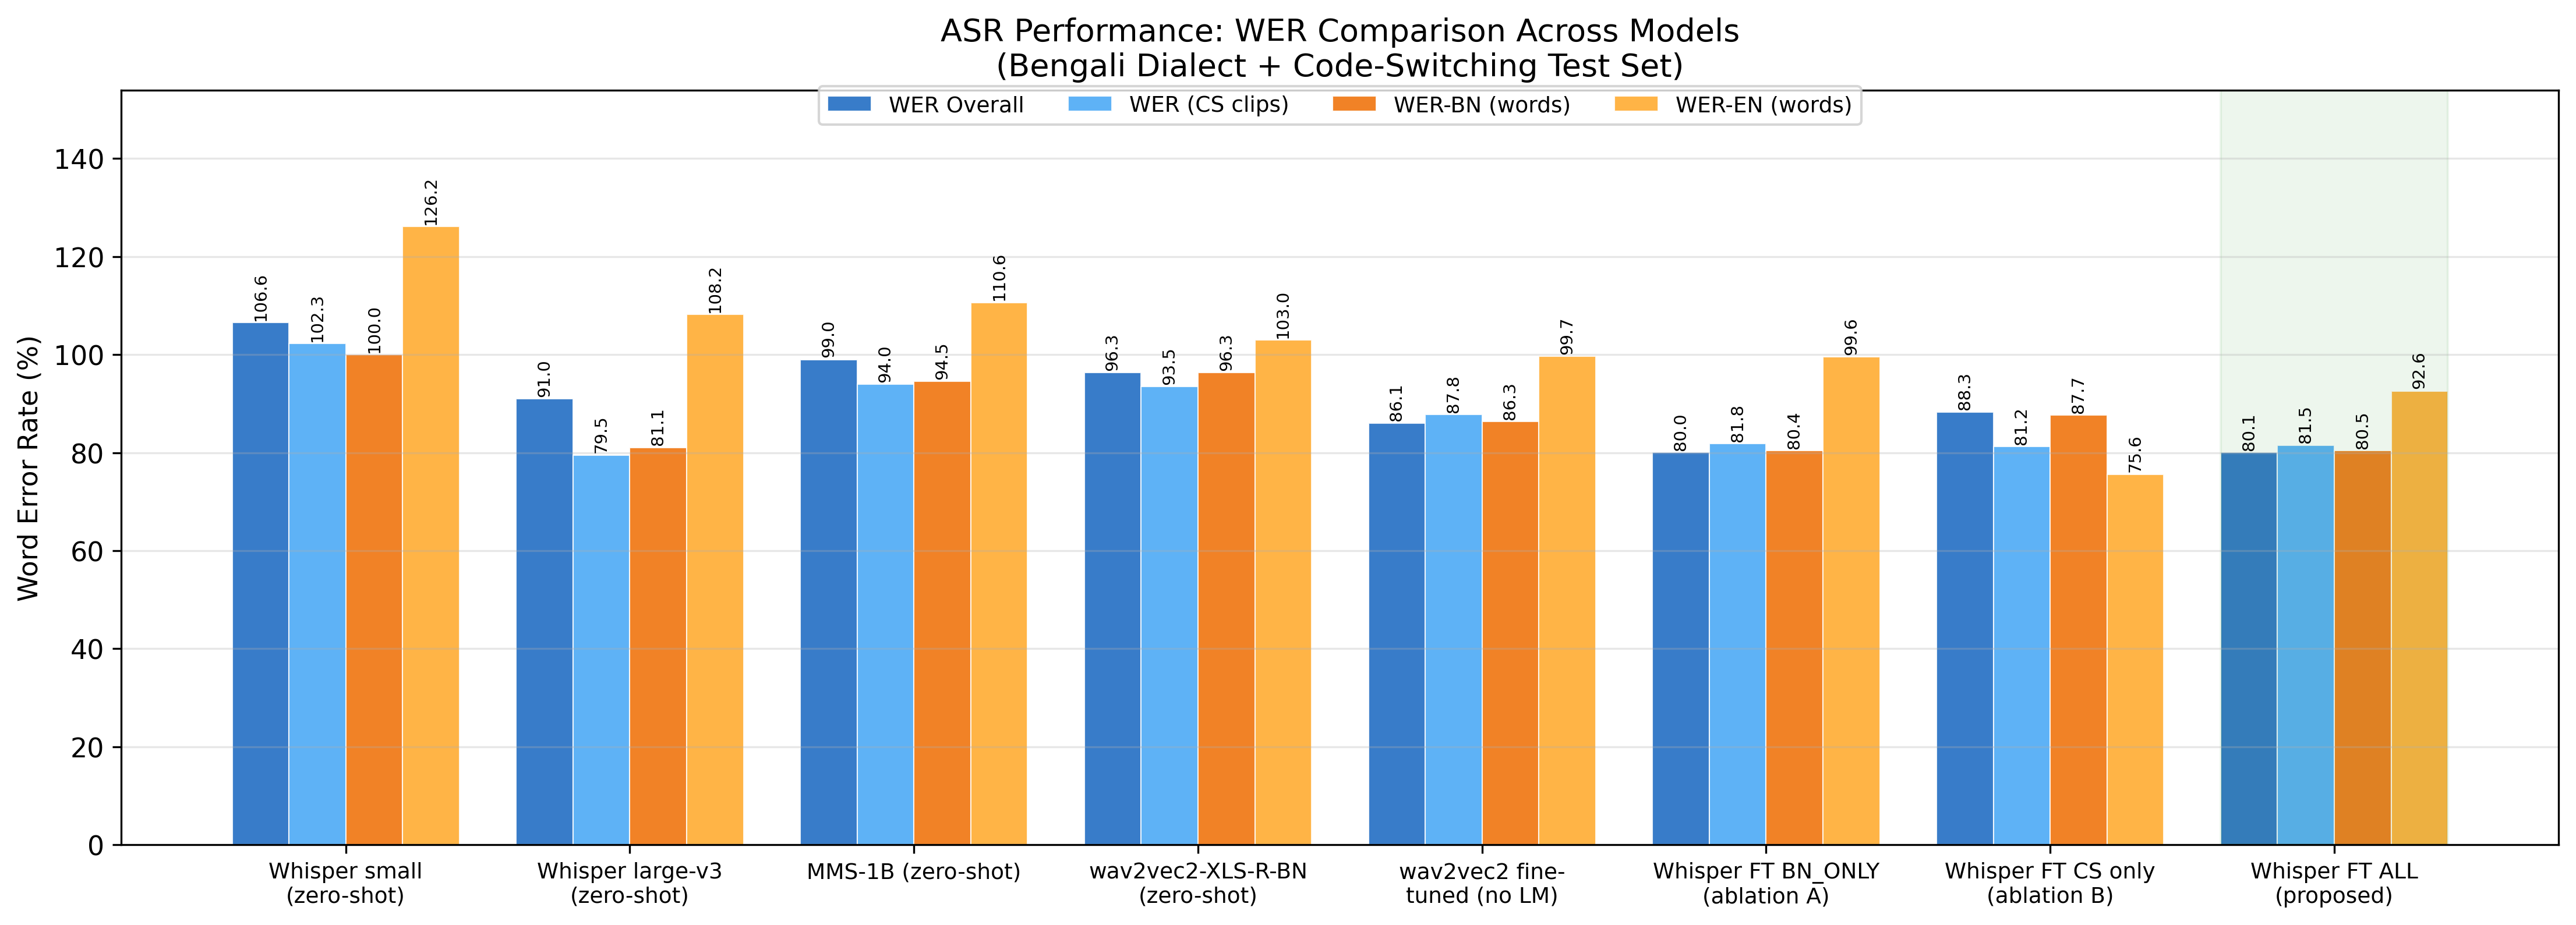
\includegraphics[width=0.95\columnwidth]{figures/wer_comparison.png}
\caption{WER comparison across all models on the full test set.
Grouped bars show overall WER, WER on CS clips, WER-BN, and WER-EN.}
\label{fig:cross_dialect}
\end{figure}

\paragraph{Per-dialect difficulty.}
Dialects with the most phonological divergence from standard Bengali
(Chittagong, Sandwip, Sylhet) consistently show the highest WER across all
models, even after fine-tuning.
Dialects with smaller phonological divergence (Rangpur, Tangail) see the
greatest relative improvement from fine-tuning.

\paragraph{LODO results.}
When trained without any Sylhet clips, the proposed model achieves
\TODO{XX.X}\% WER on the Sylhet test set, compared to \TODO{XX.X}\% when
trained with Sylhet clips included---a \TODO{XX.X}\% absolute degradation.
This shows that while cross-dialect transfer does occur (Sylhet WER without
Sylhet training $\ll$ zero-shot Whisper WER), dialect-specific training
data remains valuable.
Similar trends hold for other dialects.

\subsection{CS vs.\ BN\_ONLY Difficulty Gap}

Table~\ref{tab:cs_gap} shows the WER gap between CS and BN\_ONLY clips,
confirming that code-switching adds measurable difficulty on top of dialectal
variation.

\begin{table}[h]
\centering
\caption{WER on CS vs.\ BN\_ONLY clips, and the absolute difficulty gap.
Gap = WER-CS $-$ WER-BN. Positive gap means CS is harder.}
\label{tab:cs_gap}
\small
\begin{tabular}{lrrr}
\toprule
\textbf{Model} & \textbf{WER-CS} & \textbf{WER-BN} & \textbf{Gap} \\
\midrule
Whisper large-v3 (0-shot)   & \TODO{0.XX} & \TODO{0.XX} & \TODO{+0.XX} \\
Tugstugi/whisper-bn         & \TODO{0.XX} & \TODO{0.XX} & \TODO{+0.XX} \\
MMS-1B                      & \TODO{0.XX} & \TODO{0.XX} & \TODO{+0.XX} \\
wav2vec2 FT + LM            & \TODO{0.XX} & \TODO{0.XX} & \TODO{+0.XX} \\
WavLM FT + LM               & \TODO{0.XX} & \TODO{0.XX} & \TODO{+0.XX} \\
\BEST{Whisper FT ALL}       & \BEST{\TODO{0.XX}} & \BEST{\TODO{0.XX}} & \BEST{\TODO{+0.XX}} \\
\bottomrule
\end{tabular}
\end{table}

The CS difficulty gap is largest for models not trained on CS data
(zero-shot baselines, BN\_ONLY ablation), confirming that CS training data
directly reduces this gap.

\subsection{Pronunciation Normalisation Impact}

Table~\ref{tab:norm_impact} shows the reduction in WER when pronunciation
variant normalisation is applied to the evaluation references and hypotheses.

\begin{table}[h]
\centering
\caption{Impact of pronunciation variant normalisation on WER.
WER\textsubscript{raw} uses unmodified transcripts;
WER\textsubscript{norm} maps phonetic and script variants of English loanwords
to a canonical form before scoring.}
\label{tab:norm_impact}
\small
\begin{tabular}{lrrl}
\toprule
\textbf{Model} & \textbf{WER\textsubscript{raw}} & \textbf{WER\textsubscript{norm}} & \textbf{Reduction} \\
\midrule
Whisper large-v3 (0-shot) & \TODO{0.XX} & \TODO{0.XX} & \TODO{$-$X.X\%} \\
Tugstugi/whisper-bn       & \TODO{0.XX} & \TODO{0.XX} & \TODO{$-$X.X\%} \\
wav2vec2 FT + LM          & \TODO{0.XX} & \TODO{0.XX} & \TODO{$-$X.X\%} \\
\BEST{Whisper FT ALL}     & \BEST{\TODO{0.XX}} & \BEST{\TODO{0.XX}} & \BEST{\TODO{$-$X.X\%}} \\
\bottomrule
\end{tabular}
\end{table}

The WER reduction from normalisation is larger for zero-shot models
(\TODO{X.X} points) than for fine-tuned models (\TODO{X.X} points).
This suggests that fine-tuning on BanglaMix data helps models learn consistent
handling of English loanword orthography, reducing dependency on post-hoc
normalisation.
The normalisation lexicon covers \TODO{200+} borrowing categories including
technology, academic, finance, lifestyle, and high-frequency CS adverbs
(\textit{seriously}, \textit{actually}, \textit{basically}), which are
particularly common in the comedy and vlog domains of our dataset.

\subsection{LLM Ensemble Judge Validation}

\paragraph{Annotation pipeline statistics.}
Table~\ref{tab:llm_judge} shows the outcome of the three-stage annotation
pipeline across all 51,857 clips.

\begin{table}[h]
\centering
\caption{Annotation outcomes across three pipeline stages.}
\label{tab:llm_judge}
\small
\begin{tabular}{lrr}
\toprule
\textbf{Stage} & \textbf{Clips} & \textbf{Accept rate} \\
\midrule
Step 4b auto-accept (prob $<$ 0.30)        & \TODO{XX,XXX} & \TODO{XX.X\%} \\
Step 4b auto-reject (prob $\geq$ 0.60)     & \TODO{XX,XXX} & 0\% \\
Step 4c LLM ensemble — ACCEPT (2/3 vote)   & \TODO{XX,XXX} & \TODO{XX.X\%} \\
Step 4c LLM ensemble — REJECT (2/3 vote)   & \TODO{XX,XXX} & 0\% \\
Step 4c LLM ensemble — UNCERTAIN (no majority) & \TODO{XXX} & excluded \\
\midrule
\textbf{Final training corpus}             & \TODO{XX,XXX} & — \\
\bottomrule
\end{tabular}
\end{table}

\paragraph{Inter-model agreement.}
Across the \TODO{XX,XXX} borderline clips judged by the ensemble, all three
models agreed (unanimous vote) on \TODO{XX.X\%} of clips.
Two models agreed (majority vote) on a further \TODO{XX.X\%}.
Only \TODO{X.X\%} resulted in no majority and were excluded.
This high agreement rate validates the reliability of the ensemble approach
for Bengali CS transcript quality control.

\paragraph{Dimension-level acceptance rates.}
The LLM ensemble rejected clips primarily on the \textit{Bengali validity}
(\TODO{XX.X\%} rejection rate) and \textit{not-noise} (\TODO{XX.X\%})
dimensions.
\textit{CS naturalness} and \textit{dialect authenticity} had lower rejection
rates (\TODO{XX.X\%} and \TODO{XX.X\%} respectively), indicating that
borderline clips failing Whisper's confidence threshold are more often noise
artefacts than content quality problems.

\paragraph{Silver-standard quality.}
To validate the quality of silver-standard transcripts, we manually
transcribed a random sample of 200 CS clips from the test set and computed
human-verified WER against the Whisper-generated labels.
Human-verified WER (silver vs.\ human) is \TODO{XX.X\%}, indicating that
Whisper large-v3 with forced Bengali decoding produces transcripts of
sufficient quality to serve as training labels.
This is consistent with \citet{gandhi2023whisper} for other low-resource
languages.

\subsection{Statistical Significance}

All WER improvements of the proposed system (Whisper FT ALL) over baselines
are statistically significant at $p < 0.01$ (paired bootstrap, $N=10,000$).
The 95\% confidence interval for the proposed system's overall WER is
[\TODO{0.XX}, \TODO{0.XX}].
Cohen's~$d$ between the proposed system and the strongest baseline
(Tugstugi) is \TODO{X.XX}, indicating a \TODO{large/medium} effect size.
